 % TO DELETE

    \documentclass[journal,a4paper]{IEEEtran}
 %    \documentclass[10pt,twocolumn,twoside]{IEEEtran}
%     \documentclass[11pt,draftcls,onecolumn,peerreview]{IEEEtran} 
%         \topmargin       -6.0mm
%          \oddsidemargin      0mm
%          \evensidemargin     0mm
%          \textheight     223.5mm
%         \textwidth      170.0mm

\usepackage{color}
\newcommand{\mike}[1]{\textsf{\emph{\textbf{\textcolor{red}{#1}}}}} 
\newcommand{\dean}[1]{\textsf{\emph{\textbf{\textcolor{green}{#1}}}}} 
\newcommand{\parham}[1]{\textsf{\emph{\textbf{\textcolor{blue}{#1}}}}} 
\newcommand{\ken}[1]{\textsf{\emph{\textbf{\textcolor{magenta}{#1}}}}} 
\newcommand{\cut}[1]{\textcolor{cyan}{#1}} 

\usepackage{cite}

\ifCLASSINFOpdf
   \usepackage[pdftex]{graphicx}
  % declare the path(s) where your graphic files are
  % \graphicspath{{../pdf/}{../jpeg/}}
  % and their extensions so you won't have to specify these with
  % every instance of \includegraphics
  % \DeclareGraphicsExtensions{.pdf,.jpeg,.png}
\else
  % or other class option (dvipsone, dvipdf, if not using dvips). graphicx
  % will default to the driver specified in the system graphics.cfg if no
  % driver is specified.
  \usepackage[dvips]{graphicx}
  % declare the path(s) where your graphic files are
  % \graphicspath{{../eps/}}
  % and their extensions so you won't have to specify these with
  % every instance of \includegraphics
  % \DeclareGraphicsExtensions{.eps}
\fi

\usepackage[cmex10]{amsmath}
\interdisplaylinepenalty=2500
\usepackage{amssymb}
\ifCLASSOPTIONcompsoc
  \usepackage[tight,normalsize,sf,SF]{subfigure}
\else
  \usepackage[tight,footnotesize]{subfigure}
\fi


\usepackage{stfloats}
\usepackage{float}
\floatstyle{ruled}
\newfloat{algorithm}{htbp}{loa}%[chapter]
\floatname{algorithm}{Algorithm}

\begin{document}
%
% paper title
% can use linebreaks \\ within to get better formatting as desired
\title{Multiresolution Neural Field Estimation }
%
%
% author names and IEEE memberships
% note positions of commas and nonbreaking spaces ( ~ ) LaTeX will not break
% a structure at a ~ so this keeps an author's name from being broken across
% two lines.
% use \thanks{} to gain access to the first footnote area
% a separate \thanks must be used for each paragraph as LaTeX2e's \thanks
% was not built to handle multiple paragraphs
%

\author{In no particular order: \parham{P. Aram}, \mike{M. Dewar}, \dean{D.R. Freestone}, \ken{K.Scerri}, D.B. Grayden and V. Kadirkamanathan % <-this % stops a space
\thanks{P. Aram* and V. Kadirkamanathan are with the Department of Automatic Control and Systems Engineering, University of Sheffield, Sheffield, S1 3JD, U.K. (e-mail:p.aram@sheffield.ac.uk; visakan@sheffield.ac.uk).}% <-this % stops a space
\thanks{M. Dewar is with the School of Informatics, University of Edinburgh, Edinburgh, EH8 9AB, U.K. (e-mail:mike.dewar@inf.ed.ac.uk)}
\thanks{D.\ R.\ Freestone and D.\ B.\ Grayden are with the Department
of Electrical and Electronic Engineering, The University of Melbourne, and The Bionic Ear Institute, VIC, Australia,  {\tt\small dfreestone@bionicear.org, grayden@unimelb.edu.au}}}% <-this % stops a space
%\thanks{Manuscript received April 19, 2005; revised January 11, 2007.}}

% note the % following the last \IEEEmembership and also \thanks - 
% these prevent an unwanted space from occurring between the last author name
% and the end of the author line. i.e., if you had this:
% 
% \author{....lastname \thanks{...} \thanks{...} }
%                     ^------------^------------^----Do not want these spaces!
%
% a space would be appended to the last name and could cause every name on that
% line to be shifted left slightly. This is one of those "LaTeX things". For
% instance, "\textbf{A} \textbf{B}" will typeset as "A B" not "AB". To get
% "AB" then you have to do: "\textbf{A}\textbf{B}"
% \thanks is no different in this regard, so shield the last } of each \thanks
% that ends a line with a % and do not let a space in before the next \thanks.
% Spaces after \IEEEmembership other than the last one are OK (and needed) as
% you are supposed to have spaces between the names. For what it is worth,
% this is a minor point as most people would not even notice if the said evil
% space somehow managed to creep in.



% The paper headers
% \markboth{Journal of }%
% {Aram \MakeLowercase{\textit{et al.}}: Wavelet Multiresolution Spatio-Temporal Modelling Using the Integro-Difference Equation}
% The only time the second header will appear is for the odd numbered pages
% after the title page when using the twoside option.
% 
% *** Note that you probably will NOT want to include the author's ***
% *** name in the headers of peer review papers.                   ***
% You can use \ifCLASSOPTIONpeerreview for conditional compilation here if
% you desire.
 \ifCLASSOPTIONpeerreview
\else
\fi



% If you want to put a publisher's ID mark on the page you can do it like
% this:
%\IEEEpubid{0000--0000/00\$00.00~\copyright~2007 IEEE}
% Remember, if you use this you must call \IEEEpubidadjcol in the second
% column for its text to clear the IEEEpubid mark.



% use for special paper notices
%\IEEEspecialpapernotice{(Invited Paper)}




% make the title area
\maketitle


\begin{abstract}
%\boldmath
The Integro-difference equation (IDE) is an increasingly popular model of spatio-temporal processes. Here we develop a multiresolution approximation (MRA) framework for the IDE neural field equations based on semi-orthogonal cardinal B-spline wavelets. State and parameter estimation is approached in a Maximum Likelihood (ML) framework using the Expectation Maximisation (EM) algorithm. Examples are given to demonstrate the framework.
\end{abstract}

% Note that keywords are not normally used for peerreview papers.
\begin{IEEEkeywords}
Neural field model, multiresolution approximation (MRA), Expectation Maximization (EM) algorithm, wavelets.
\end{IEEEkeywords}






% For peer review papers, you can put extra information on the cover
% page as needed:
% \ifCLASSOPTIONpeerreview
%  \begin{center} \bfseries EDICS Category: SSP-IDEN \end{center}
%  \fi
%
% For peerreview papers, this IEEEtran command inserts a page break and
% creates the second title. It will be ignored for other modes.
\IEEEpeerreviewmaketitle

% We have a clear definition and where to stimulate and how to stimulate.\\
% \cut{This color is used to indicate bits we can get rid of if we don't have enough space, use the command: \textbackslash cut$\left\lbrace  \right\rbrace$}

\section{Introduction}
\IEEEPARstart{T}{he} human brain has a multiresolution architecture, where spatial scales for information processing and transfer range from individual proteins in synapses, to neurons, to networks of neurons. The multiresolution cortical architecture poses major modeling challenges to efficiently describe the brain's dynamics. This paper introduces a multiresolution data-driven framework for neural field modeling, the multiresolution approximate integrodifference equation (MRAIDE), to address this challenge. 

Neural field models typically describe the meso and macroscopic dynamics of the human brain, but are also descriptive of finer-scale neurodynamics. The ability to create patient-specific neural models will contribute to our knowledge base of poorly understood diseases such as epilepsy, and furthermore, may also enable the development of new treatment strategies. This is particularly poignant with the advent of new devices that use therapeutic electrical stimulation. Presently, stimulation strategies for devices operate in an open-loop, where stimulation parameters are chosen using a process of trial and error. Therefore, there exists an enormous potential to improve the performance of these devices using systems theory. The design of a stimulation strategy using systems theory requires a model. Neural mass and neural field models are the ideal candidates for estimation and control algorithms. It is expected that parameters of the neural fields models will be patient specific and will therefore need to be inferred from data.

The first work describing data driven mesoscopic neural modeling~\cite{Valdes1999} used a neural mass model~\cite{LopesDaSilva1976,Zetterberg1978} to fit EEG data. This approach was extended to coupled neural masses (using another model~\cite{Jansen1995}) through a Bayesian estimation scheme dubbed Dynamic Causal Modeling (DCM)~\cite{David2003}. Following this work, data-driven modeling was extended to continuum field equations that explain the richer dynamics of spatiotemporal neural fields \cite{Galka2008,schiff2008kalman,Daunizeau2009}. Most recently a framework was developed where a finite element model of the neural field (via a global Galerkin projection) was formed, using a basis function decomposition, to transform the PDE neural field equations into a finite dimension system to facilitate efficient state and parameter estimation~\cite{Freestone2011}.  

This paper is an extension to this recent study~\cite{Freestone2011}. The basis function decomposition in this previous study did not account for multiresolution architecture and spatial dynamics of the human cortex. Thus, it can be improved.. In this current paper, a multiresolution approach is taken...

By taking the multiresolution approach, the identified IDE model will approximate the underlying spatio-temporal dynamics at different spatial scales. In this way both macroscopic and microscopic behaviour of the system can be represented simultaneously...

\section{Integro-Difference Equation Neural Field Model}
The stochastic integro-difference equation (IDE) form of the Amari neural field  formulation~\cite{Amari1977} is given by (see~\cite{Freestone2011} for a full derivation)
\begin{equation}\label{eq:DiscreteTimeModel}
	v_{t+T_s}\left(\mathbf{r}\right) = 
	\xi v_t\left(\mathbf{r}\right) + 
	T_s \int_\Omega { 
	    w\left(\mathbf{r},\mathbf{r'}\right)
	    f\left(v_t\left(\mathbf{r}'\right)\right) 
	\, d\mathbf{r}'} 
	+ e_t\left(\mathbf{r}\right), 
\end{equation}
where the post-synaptic membrane voltage at time $t$ of a population of neurons at position $\mathbf r$ is denoted $v_t\left(\mathbf r\right)$. Synaptic dynamics are included through the parameter $\xi=\left(1-\frac{ T_s}{\tau}\right)$, where $\tau$ is the synaptic time constant and $T_s$ is the sampling time. The connectivity strength between neural populations at a distance $\mid\mathbf{r}-\mathbf{r'}\mid$ is described by the kernel $w\left(\mathbf{r}-\mathbf{r}'\right)$. The connectivity kernel is taken as a ``Mexican hat'' function, which describes local excitation and lateral inhibition \cite{Amari1977}. The term $e_t(\mathbf r)$ is an $i.i.d.$ disturbance such that $e_t(\mathbf{s})\sim\mathcal{GP}(\mathbf 0,\eta(\mathbf{r}-\mathbf{r'}))$, where $\mathcal{GP}(\mathbf 0,\eta(\mathbf{r}-\mathbf{r'}))$  denotes a zero mean spatial Gaussian process with covariance function $\eta(\mathbf{r}-\mathbf{r'})$~\cite{Rasmussen2005}. For simplicity, \cut{we denote the current time step by $t$ and the future time step by $t+1$.} The firing rate of the presynaptic neurons is related to the post-synaptic membrane potential by the activation function $f\left(.\right)$. \dean{The activation function is of the form $f(v_t(\mathbf{r})) = \varsigma v_t(\mathbf{r}) + v_0$}. A linear form of the activation function was chosen to construct the estimator due to high computational demands when using a nonlinear (sigmoidal) activation function.

The observation equation describing the electrophysiological recordings is given by 
\begin{equation}\label{eq:ObservationEquation}
	\mathbf y_t = \int_{\Omega} { m\left(\mathbf{r}_{n_y}-\mathbf{r}'\right) v_t\left(\mathbf{r}'\right) \, d\mathbf{r}'} + \boldsymbol\epsilon_t, 
\end{equation}
where $\mathbf{y}_{t} = [y_t(\mathbf{r}_1) y_t(\mathbf{r}_2) \cdots y_t(\mathbf{r}_{n_y})]^\top$, compiled at $n_{y}$ spatial locations at time $t$ via the observation kernel $m\left(\mathbf{r}_{n_y}-\mathbf{r}'\right)$, is corrupted by an i.i.d normally distributed zero-mean white noise $\boldsymbol{\epsilon}_{t}\sim \mathcal{N}\left(\mathbf{0},\mathbf{\Sigma}_{\epsilon}\right)$ with $\mathbf{\Sigma}_{\epsilon}=\sigma_{\epsilon}^2\mathbf I_{n_y} $. The superscript $\top$ denotes the transpose operator.

\section{MRA of the IDE in State-Space}
The multiresolution approximation (MRA) of the neural IDE is obtained by decomposing both the field, $v_t(.)$, and the connectivity kernel, $w(.)$, (assuming square-integrable functions) using translations and dilations of a scaling function $\phi(\mathbf{r})$ and a mother wavelet $\psi(\mathbf{r})$. Considering a one-dimensional field, the connectivity kernel is decomposed by,
\begin{equation}
 w\left(r-r'\right)=\sum_{l \in \mathbb{Z}}\alpha_{j_0,l}\phi_{j_0,l}\left(r-r'\right)+\sum_{j\geq j_0}^{\infty} \sum_{l \in \mathbb{Z}}\beta_{j,l}\psi_{j,l}\left(r-r'\right), 
\label{eq:KernelExpansion}
\end{equation}
where $\alpha_{j_0,l}$ are the approximation coefficients at the lowest scale $j_0$, and $\beta_{j,l}$ are the detail coefficients at different scales $j$, with $\phi_{j,l}\left(r\right)=2^{\frac{j}{2}}\phi\left(2^jr-l\right) $ and $\psi_{j,l}\left(r\right)=2^{\frac{j}{2}}\psi\left(2^jr-l\right)$. Integers $j$ and $l$ are the scale and translation parameters respectively. The field is decomposed as
\begin{equation}
 v_t\left(r\right)=\sum_{l \in \mathbb{Z}}x_{t,j_{0},l}\phi_{j_{0},l}\left(r\right)+\sum_{j\geq j_0}^{\infty} \sum_{l \in \mathbb{Z}} \check{x}_{t,j,l}\psi_{j,l}\left(r\right),
\label{eq:FieldExpansion}
\end{equation}
where $ x_{t,j_{0},l}$ and $\check{x}_{t,j,l} $ are the coefficients of the expansion at time $t$.

Eqs. \eqref{eq:KernelExpansion} and \eqref{eq:FieldExpansion} are infinite series expansions, but  for a practical implementation they must be truncated at some level $j$. Therefore, the field and the connectivity kernel is approximated by
 \begin{align}
 w\left(r-r'\right) &\approx \boldsymbol\theta^\top\boldsymbol\lambda\left(r-r'\right) 
\label{eq:KernelFiniteExpansion} \\
 v_t\left(r\right) &\approx \boldsymbol\mu\left(r\right)^\top\mathbf{x}_t,
\label{eq:FieldFiniteExpansion}
\end{align}
where the unknown parameter and state vectors, $\boldsymbol\theta \in \mathbb{R}^{n_{\theta}}$ and $\mathbf{x}_t \in \mathbb{R}^{n_x}$, are defined as 
\begin{align}
 \boldsymbol\theta^\top &=\left[ \boldsymbol\alpha_{j_0}^\top \quad \boldsymbol\beta_{j_0}^\top \quad \boldsymbol\beta_{j_0+1}^\top \cdots \boldsymbol\beta_{j}^\top\right] 
\label{KernelWeights} \\
 \mathbf{x}_{t}^\top &=\left[\mathbf{x}_{t,j_{0}}^\top \quad  \check{\mathbf{x}}_{t,j_{0}}^\top \quad  \check{\mathbf{x}}_{t,j_{0}+1}^\top \cdots \check{\mathbf{x}}_{t,j}^\top\right].
\label{FieldWeights}
\end{align}
The kernel and field approximation coefficient vectors $\boldsymbol \alpha_{j_0}$ and $\mathbf{x}_{t,j_{0}}$ contain all the coefficients $\left\lbrace\alpha_{j_0, l}:l \in \mathbb{Z} \right\rbrace $ and $\left\lbrace x_{t,j_0, l}: l \in \mathbb{Z}\right\rbrace$, respectively. Similarly, the kernel and the field detail coefficient vectors, $\boldsymbol\beta_{j}$ and $\check{\mathbf{x}}_{t,j}$ contain all the coefficients $\left\lbrace \beta_{j,l} :l \in \mathbb{Z}\right\rbrace$ and $\left\lbrace  \check x_{t,j, l}:l \in \mathbb{Z}\right\rbrace$ respectively.

The vectors of the kernel and the field scaling and wavelet functions, $\boldsymbol\lambda$ and $\boldsymbol\mu$ respectively, are defined by
\begin{align}
 \boldsymbol\lambda^\top & (r-r')=\left[ \boldsymbol\phi_{j_0}^\top(r-r') \quad \boldsymbol\psi_{j_0}^\top(r-r') \quad \boldsymbol\psi_{j_0+1}^\top(r-r') \right. \nonumber \\
&\left. \cdots \quad \boldsymbol\psi_{j}^\top(r-r')\right] \label{KernelBasisVector} \\
 \boldsymbol\mu^\top & (r)=\left[ \boldsymbol\phi_{j_0}^\top(r) \quad \boldsymbol\psi_{j_0}^\top(r) \quad \boldsymbol\psi_{j_0+1}^\top(r) \cdots \boldsymbol\psi_{j}^\top(r) \right]. 
\label{FieldBasisVector}
\end{align}
The vectors in Eqs. (\ref{KernelBasisVector}) and (\ref{FieldBasisVector}) are constructed in the same manner as the vectors in Eqs. (\ref{KernelWeights}) and (\ref{FieldWeights}). 

To derive the state-space model, Eqs.~\eqref{eq:KernelFiniteExpansion} and \eqref{eq:FieldFiniteExpansion} are substituted into Eq. \eqref{eq:DiscreteTimeModel}, then we cross-multiply by $\boldsymbol\mu\left(\mathbf r\right)$ and integrate over the space giving
\begin{align}\label{eq:DecomposedModel2} 
	&\int_{\Omega} \boldsymbol\mu  \left(r\right)\boldsymbol\mu\left(r\right)^\top  dr\mathbf{x}_{t+1}= 
	\xi\int_{\Omega}\boldsymbol\mu\left(r\right)\boldsymbol\mu\left(r\right)^\top d\mathbf{r}\mathbf{x}_t \nonumber \\
	&+T_s \int_{\Omega}\boldsymbol\mu\left(r\right) \int_\Omega { 
	   \boldsymbol\theta^\top\boldsymbol\lambda\left(r-r'\right)
	    \boldsymbol\mu^\top\left(r'\right)\mathbf{x}_t 
	\, dr'd\mathbf{r}} \nonumber \\
	+& \int_{\Omega}\boldsymbol\mu\left(r\right)e_t\left(r\right)dr.
\end{align}
In order to simplify the model we define the matrices
\begin{align}\label{eq:Lambdax}
 \mathbf{\Lambda}_{x} &\triangleq \int_{\Omega}\boldsymbol\mu\left(r\right)\boldsymbol\mu^\top\left(r\right) dr \\
\label{eq:Lambdatheta}
 \mathbf{\Lambda}_{\theta} &\triangleq \int_{\Omega}\boldsymbol\mu\left(r\right) \int_\Omega { 
	   \boldsymbol\theta^\top\boldsymbol\lambda\left(r-r'\right)
	    \boldsymbol\mu^\top\left(r\right)\mathbf{x}_t 
	\, dr'dr}
\end{align}
and substitute them into Eq.~\eqref{eq:DecomposedModel2}. Then we cross-multiply by $\mathbf{\Lambda}_{x}^{-1}$ giving
\begin{align}\label{eq:StateEquation}
 \mathbf x_{t+1} &=\mathbf A(\boldsymbol \theta) \mathbf x_t+ \mathbf w_t \\
\label{eq:A_theta}
 \mathbf A(\boldsymbol \theta) &= (T_s\mathbf{\Lambda}_{x}^{-1}\mathbf{\Lambda}_{\theta}+\xi\mathbf I),
\end{align}
where $\mathbf I$ is the identity matrix. The disturbance becomes 
\begin{equation}\label{eq:Disturbance}
\mathbf w_t= \mathbf{\Lambda}_{x}^{-1}\int_{\Omega}\boldsymbol\mu \left(\mathbf{r}\right)e_t\left(\mathbf{r}\right)d\mathbf{r},
\end{equation}
which is a vector valued, zero-mean normally distributed white noise process with covariance (see \cite{Scerri2009} for proof)
\begin{equation}
\boldsymbol\Sigma_w =\mathbf{\Lambda}_{x}^{-1}\iint\limits_{\boldsymbol\Omega}\boldsymbol\mu\left(r\right) \eta\left(r-r'\right)\boldsymbol\mu^{\top}\left(r'\right)dr'dr\mathbf{\Lambda}_{x}^{-\top}.
\end{equation}
The observation equation of the state-space model is found by substituting decomposition \eqref{eq:FieldFiniteExpansion}
 into equation \eqref{eq:ObservationEquation} giving
\begin{equation}\label{eq:ReducedObservationEquation} 
	\mathbf{y}_t = \mathbf{C}\mathbf{x}_t + \boldsymbol{\varepsilon}_t,
\end{equation}
where each element of the observation matrix is given by
\begin{equation}
	\mathbf{C}_{ij} \triangleq \int_{\Omega}m(\mathbf{r}_i - \mathbf{r}')\boldsymbol{\mu}_j(\mathbf{r}') \, d\mathbf{r}'.
\end{equation}
This completes derivation of the state-space representation of the multiresolution approximation of the neural field model. 
% \parham{Mike you can add state-space derivation using Galerkin projection here.}

The multiresolution approximation can be implemented using various classes of scaling and wavelet functions. B-spline functions were chosen due their compact support and the ability to analytically calculate convolution and inner product to form the matrices $ \boldsymbol\Lambda_x$ and $\boldsymbol \Lambda_{\theta}$. To show how the matrices are formed, the $m^{th}$ order cardinal B-spline scaling function is defined by the recurrence relation \cite{Chui1992} 
\begin{align}
N_{m}\left(r\right)=&\left(N_{m-1}\ast N_{1}\right)\left(r\right)\nonumber \\
=&\int_0^{1} N_{m-1}\left( r-r'\right)dr' \quad m>1,
\label{SplineConvolutionIntegral}
\end{align}
where $\ast$ denotes convolution and $N_1\left(s\right)$ is the characteristic function of the unit interval $\left[ 0,1\right)$
\begin{equation}
N_{1}\left(r\right)=
\begin{cases}
1 & \text{if $ 0\le r<1$}, \\
0 & \mathrm{elsewhere}.
\end{cases}
\end{equation}
Eq.~\ref{SplineConvolutionIntegral} can be rewritten as $(m-1)$ times convolution of indicator function with itself since
\begin{equation}
 N_{m}\left(r\right)=\underbrace{\left(N_{1}\ast N_{1}\ast \cdots \ast N_{1}\right)}_{m-1\quad \text{convolutions}}\left(r\right).
\end{equation}
Using the associativity property of convolution we have
\setlength{\arraycolsep}{0.0em}
\begin{align}\label{eq:BsplineConvolution}
N_{m}\left( r\right) \ast N_{m'}\left(r\right)&=\underbrace{\overbrace{\left(N_{1} \ast \cdots \ast N_{1}\right)}^{m-1 \quad \text{convolutions}}\left(r\right) \ast \overbrace{\left(N_{1} \ast \cdots \ast N_{1}\right)}^{m'-1\quad \text{convolutions}}}_{m+m'-1 \quad \text{convolutions}}\left(r\right)\nonumber\\
&=N_{m+m'}\left(r\right).
\end{align}
A direct consequence of Eq.~\eqref{eq:BsplineConvolution} is (see \cite{Chui1992} for proof) 
\begin{align}
 \left\langle N_{m}\left(r-l_{1}\right), N_{m'}\left(r-l_{2}\right)\right\rangle=&N_{m+m'}\left(m+l_{1}-l_{2}\right)\nonumber \\
=&N_{m+m'}\left(m'+l_{2}-l_{1}\right),
\label{eq:BsplineInnerProduct}
\end{align}
where $\left\langle \cdot,\cdot\right\rangle $ denotes the inner product. The $m^{th}$ order B-spline wavelet function is defined as (see \cite{Chui1992}) 
\begin{align}
 \varphi & _{m}\left(r\right) = \sum_{n=0}^{3m-2} q_n N_{m}\left(2r-n\right) \\
 q & _n = \frac{\left(-1\right)^n}{2^{m-1}} \sum_{l=0}^{m} \binom{m}{l} N_{2m}\left(n-l+1\right), \,  \text{ $0\le n\le 3m-2$},
\end{align}
where $q_n$ are the coefficients. By exploiting properties Eqs.~\ref{eq:BsplineConvolution} and \ref{eq:BsplineInnerProduct} the integrals in Eqs.~\ref{eq:Lambdax} and \ref{eq:Lambdatheta} can be computed. In order to calculate elements of $\boldsymbol\Lambda_{x}$ and $\boldsymbol\Lambda_{\theta}$ the scaling and wavelet basis functions must be expanded in terms of $N_m$ at the appropriate scale.  In this paper $4^{th}$ order cardinal B-spline scaling and wavelet functions are used. Therefore, the $8^{th}$ and $12^{th}$ order B-spline values at integer points are required (see \cite{Goswami1999}) to compute the integrals in Eqs.~\ref{eq:Lambdax} and \ref{eq:Lambdatheta}.

\section{State and Parameter Estimation}
The state-space representation of the MRAIDE allows the use of the well known Expectation Maximization (EM) algorithm \cite{Dempster1977} to infer both the kernel and the field from electrophysiological data. The EM algorithm, when used to in this context \cite{Dewar2009}, yields the maximum likelihood kernel estimate and the posterior distribution of the field over time. We use the standard EM algorithm for linear dynamic systems \cite{Gibsona2005,Roweis1999,Shumway2000} and hence only describe aspects of the algorithm that are specific to MRA neural field equations. EM essentially finds increasingly tighter lower bounds on the likelihood of the kernel $p(\mathbf{y}_1 \ldots \mathbf{y}_T|w)$ so that, at convergence, the maximum of the bound corresponds to the maximum of the likelihood. For a multivariate linear dynamic system, the bound used is a quadratic of the form
\begin{equation}
 \mathcal Q\left(\boldsymbol \theta,\boldsymbol\theta'\right)=\beta+2T_s\left(\boldsymbol\upsilon_0-\boldsymbol\upsilon_1\right)\boldsymbol\theta-T_s\boldsymbol\theta^\top\boldsymbol\Upsilon\boldsymbol\theta,
\end{equation}
which has a maximum at
\begin{align}
 \boldsymbol \theta= \boldsymbol\Upsilon^{-\top}(\boldsymbol\upsilon_0^\top-\boldsymbol\upsilon_1^\top),
\end{align}
where
\begin{align}\label{eq:upsilon0}
 \boldsymbol\upsilon_0&=\sum_{i,j=1}^{n_x}[\boldsymbol\Xi_0]_{i,j}[\Sigma_{w}^{-1}\boldsymbol\Lambda_{x}^{-1}\mathbf U]_{j,i}\\ 
 \boldsymbol\upsilon_1&=\xi\sum_{i,j=1}^{n_x}[\boldsymbol\Xi_1]_{i,j}[\Sigma_{w}^{-1}\boldsymbol\Lambda_{x}^{-1}\mathbf U]_{j,i}\label{eq:upsilon1} \\
 \boldsymbol\Upsilon&=T_s\sum_{i,j=1}^{n_x}[\boldsymbol\Xi_1]_{i,j}[\mathbf{U}^{\mathsf T} \boldsymbol\Lambda_{x}^{-1}\Sigma_{w}^{-1}\boldsymbol\Lambda_{x}^{-1}\mathbf{U}]_{j,i}\label{eq:Upsilon}.
\end{align}
The $\left(i,j\right)^{th}$ block of the block matrix $\mathbf U_{n_x \times n_x}$ is given by
\mike{you need to define and sort out the $[]_{ij}$ notation!}
\begin{align}
\left[ \mathbf U\right] _{i,j}&=\int_{\boldsymbol \Omega}\left[\mu(r) \right]_i \left[\int_{\boldsymbol\Omega} \boldsymbol\mu\left(r'\right)\boldsymbol \lambda^\top \left(\mathbf{r-r'}\right) dr'\right]_{j:} dr.
\end{align}
where $[.]_{j:} $ denotes $j^{th}$ row of the matrix.%\cut{The second terms in Eqs. \ref{eq:upsilon0}, \ref{eq:upsilon1}, and \ref{eq:Upsilon} can be computed as a once-off before the commencement of the EM iterations, which increases the speed of the M-step significantly compared to the method in \cite{Dewar2009}.} 
The matrices $\Xi_0$ and $\Xi_1$ are calculated using the Rauch Tung Streibel (RTS)\cite{RAUCH1965} smoother outputs: state estimates, $\hat{\mathbf x}_t$, covariance, $\mathbf P_t=\mathrm{cov}(\mathbf{x_t})$, and cross-covariance matrix $\mathbf M_t=\mathrm{cov}(\mathbf{x}_{t-1},\mathbf{x}_{t})$ 
\begin{align}\label{eq:Xivariables}
\boldsymbol\Xi_0&=\sum_{t=0}^{T-1}\left(\mathbf M_{t+1}+\mathbf{\hat x}_t\mathbf{\hat x}_{t+1}^\top\right) \\
 \boldsymbol\Xi_1&=\sum_{t=0}^{T-1}\left(\mathbf P_t+\mathbf{\hat x}_t\mathbf{\hat x}_t^\top\right).
\end{align}
Hence, the algorithm has two distinct steps: the E-step which computes $\boldsymbol\Xi_0$ and $\boldsymbol\Xi_1$ based on the most recent parameter estimates using the RTS smoother, and the M-step which updates the paramter estimates by computing the (analytic) maximum of $Q(\theta,\theta')$. The EM algorithm iterates between these two steps until the parameter estimates converge. 


\section{Results}
To demonstrate the performance of the MRA estimation framework, data was generated synthetically  using Eqs.~\ref{eq:DiscreteTimeModel} and \ref{eq:ObservationEquation}, enabling a comparison between true and estimated parameters. 100 realizations of 1 second of data were generated where $\boldsymbol\Sigma_v=0.1 \times \mathbf{I}_{n_y}$ and $\eta(r-r')=\phi_{3,-2}(r-r')$. The sampling period and the synaptic time constant were set to $T_s = 1$~ms and $\tau = 10$~ms respectively. The distance between adjacent sensors was $0.5$~mm resulting into 161 observations. The observation kernel is modeled using a B-spline function, with a width of 0.8~mm at half the maximum amplitude of the observation kernel. The spacing and bandwidth of the sensors allowed for the full spatial bandwidth of the field to be observed. The actual connectivity kernel and its decomposition are plotted in \figurename{\ref{fig:KernelAndFreqResponse}} (a). 

The spatial frequency of the observed field is shown in \figurename{\ref{fig:KernelAndFreqResponse}} (b), showing a spatially band-limited signal. This suggests the use of wavelets up to level $j=2$ (with the bandwidth $\approx[2.5,4]$ cycles/mm) can fully represent the field. Note that wavelets due to their bandpass filter characteristics extract successively higher and higher frequency components by increasing $j$.

Field reconstruction \dean{using the results of the EM algorithm} at different levels of approximations is shown in \figurename{\ref{fig:FieldEstimates}}. \dean{Needs more info.} The figure confirms that $j=2$ is adequate to capture the dynamic of the underlying field \dean{since the error converges?}. The root mean square error (RMSE) of the field estimates is shown in \figurename{\ref{fig:ParametersHistogram}} (a). 

The histogram in \figurename{\ref{fig:ParametersHistogram}} demonstrates the performance of the parameter estimation. \dean{The results are good because the RMSE between the true and estimated kernels is $1.83$ (units?)... There is a bias of 7.4 \% in $\theta_1$ because..., which is not big deal.}
\begin{figure}[!h]
 \centering
 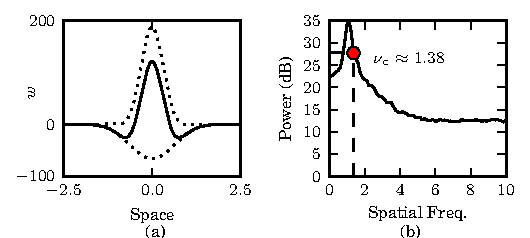
\includegraphics[scale=1]{./Graph/ObservationFreqResponse.pdf}
 \caption{(a) Mexican-hat connectivity kernel. The kernel is a composite of two B-spline
functions (dashed lines), representing local excitation and lateral inhibition. (b) The average (over time) power in dB of the spatial frequency of the observations. The dashed line shows the cutoff frequency (-3 dB point).}
\label{fig:KernelAndFreqResponse} 
  \end{figure} 
\begin{figure}[!h] 
 \centering
 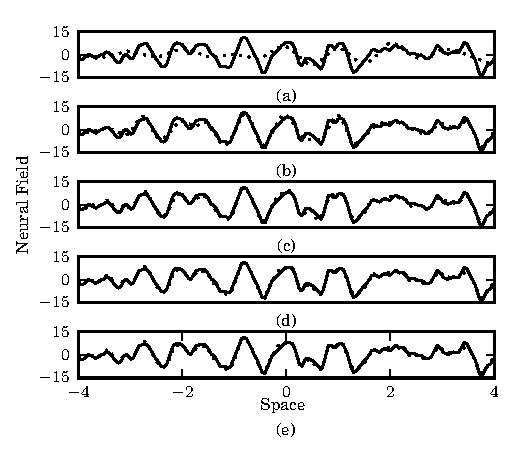
\includegraphics[scale=1]{./Graph/Field.pdf}
 \caption{Actual (solid line) and estimated (dashed line) neural fields at a time instant for different spatial resolutions. (a) $j=0$, $n_x=17$. (b) $j=1$, $n_x=33$. (c) $j=2$, $n_x=65$. (d) $j=3$, $n_x=131$. (e) $j=4$, $n_x=263$.}
 \label{fig:FieldEstimates}
 \end{figure} 
\begin{figure}[!h] 
 \centering
 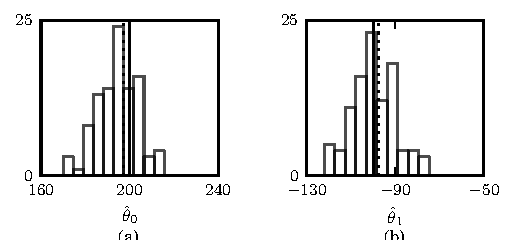
\includegraphics[scale=1]{./Graph/Hist.pdf}
 \caption{(a) RMSE of the estimated field at different spatial scales. (b-c) Histograms of the excitatory and inhibitory connectivity basis function parameter estimates, $\theta_0$ and $\theta_1$, respectively. The solid lines show the actual parameter values and the dotted lines show the means of the estimated parameters.}
 \label{fig:ParametersHistogram}
 \end{figure} 

\section{Discussion}
In this paper, we have presented a novel model-based framework for estimating cortical dynamics from electrophysiological measurements. The novel aspects include...

This work extends previous work by... alternative ARMA model... The MRA IDE can be applied to fluid dynamics, weather systems, ....

Other groups have previously highlighted the importance of a multiresolution approach in neural field modeling. For example, it is thought that the connectivity structure differs at different spatial scales, where at a fine scale a homogeneous connectivity exists and at a larger scale the connectivity become~\cite{Qubbaj2009}....

In order to apply the framework to real data several assumptions must be made, such as stationarity of the parameters over the estimation period. Perhaps the most critical assumption is that the model provides an apt description of the cortical dynamics. The authors acknowledge that there is, and will always be, a discrepancy between the model and cortex. An obvious discrepancy is, for example, the linear activation function. Nevertheless, the model-based framework proposed in this paper may enable meaningful state tracking and connectivity estimation. Furthermore, the theory presented in this paper can be adapted to more sophisticated nonlinear forms of the field equations. The key development in this paper is the multiresolution decomposition forming the state-space model, which holds for a nonlinear activation function. If a nonlinear activation function was used, then unscented RTSS should be used in the E-step of the estimation algorithm. 

Future work should be directed towards extending the framework to account heterogeneity and perhaps time delays at lower spatial resolutions. Another useful extensions would be the inclusion of a second-order synaptic response kernel to enrich the dynamics from the model. Most importantly, future work should be directed towards applying and validating the framework on real data.




% use section* for acknowledgement
%\section*{Acknowledgment}

% Can use something like this to put references on a page
% by themselves when using endfloat and the captionsoff option.
\ifCLASSOPTIONcaptionsoff
  \newpage
\fi

  \newpage
% \bibliographystyle{unsrt} 
% \bibliography{MRAIDE}

\bibliographystyle{IEEEtran}
% argument is your BibTeX string definitions and bibliography database(s)
 \bibliography{IEEEabrv,MRAIDE}


\end{document}


